\documentclass[14pt]{beamer}
\mode<presentation>
{
\usepackage{color}
\usepackage{graphicx}
\usepackage{tikz}
\usetheme[white]{Wisconsin}
\setbeamercovered{transparent}
}

\begin{document}

\title{DAG-MCNP \& make\_watertight}
\author{Patrick C Shriwise}
\institute{University of Wisconsin - Madison}
\date{December 06, 2013}

%--- Title Frame ------------%
\maketitle


%--- Frame 2 ----------------%
\begin{frame}
\frametitle{Brief History}
\begin{itemize}
\item Undergrad at Kansas State University
\item Worked on Pegasus (ST) for 2 years at UW - Madison
\item Came to CNERG in July of 2013
\vfill
\textbf{Research goal:} \\
Improve the robustness \& performance of geometry handling in DAG-MCNP\\
(watertightness, faceting, topology)
\end{itemize}
\end{frame}

%--- Frame 3 ----------------%
\begin{frame}
\frametitle{Overview}

\begin{itemize}

\item Motivation
\item Current impact of DAG-MCNP
\item DAG-MCNP workflow
\item make\_watertight algorithm
\item Examples
\item Limitations
\item Current research

\end{itemize}
\end{frame}

%--- Frame 4 ----------------%
\begin{frame}
\frametitle{Motivation for CAD-based Monte Carlo}
\begin{itemize}
\vfill
\item Faster
	\begin{itemize}
	\item faster design iteration
	\item provides a common domain inter-analysis coupling
	\end{itemize}
\vfill
\item Cheaper
	\begin{itemize}
	\item reduced human effort
	\end{itemize}
\vfill
\item Better
	\begin{itemize}
	\item avoidance of human error
	\item ability to describe higher-order surfaces
	\end{itemize}
\end{itemize}

\end{frame}

%--- Frame 5 ----------------%
\begin{frame}
\frametitle{Impact of DAG-MCNP}
\vfill
\includegraphics[scale=0.43, trim = 0 0 28 0]{QualityGraph.png}
\end{frame}

%--- Frame 6 ----------------%
\begin{frame}
\frametitle{Impact of DAG-MCNP}
\includegraphics[scale=0.43, trim = 0 0 28 0]{InitialGraphImpact.png}
\end{frame}


%--- Frame 7 ----------------%
\begin{frame}
\frametitle{DAG-MCNP Workflow}
\begin{center}
\includegraphics[scale=0.23, trim = 40 200 0 0]{DAGMC_Wrkflw1.png}
\end{center}
\end{frame}


%--- Frame 8 ----------------%
\begin{frame}
\frametitle{DAG-MCNP Workflow}
\begin{center}
\includegraphics[scale=0.23, trim = 40 200 0 0]{DAGMC_Wrkflw2.png}
\end{center}
\end{frame}

%--- Frame 9 ----------------%
\begin{frame}
\frametitle{Imprint and Merge}
\begin{itemize}
\item Imprint:
	\begin{itemize}
	\item merges coincident surfaces topologically
    \item creates a new surface for both volumes where they touch
    \item allows volumes to touch on the same surface
    \item some tolerance is allowed in this process
	\end{itemize}
\item Merge:
	\begin{itemize}
	\item merges entities that are topologically
	\textbf{and} geometrically coincident
	\item main purpose is to remove redunant definitions of curves, vertices, etc.
	\end{itemize}
\end{itemize}

\end{frame}



%--- Frame 10 ----------------%
\begin{frame}
\frametitle{DAG-MCNP Workflow}
\begin{center}
\includegraphics[scale=0.23, trim = 40 200 0 0 ]{DAGMC_Wrkflw3.png}
\end{center}
\end{frame}



%--- Frame 11 ----------------%
\begin{frame}
\frametitle{CGM \& MOAB}
\begin{itemize}
\item Common Geometry Module (CGM)
	\begin{itemize}
	\item facet-based geometry manipulation tool
	\item underlying CUBIT geomtery engine
	\item directly modifies the native CAD gometry format model
	\item avoids translation errors
	\end{itemize}
	\vfill
\item Mesh-Oriented datABase (MOAB)
	\begin{itemize}
	\item mesh manipulation and evaulation tool
	\item allows storage of metadata (material defs)
	\item PyTAPS allows for mesh manipulation through simple Python scripts
	\end{itemize}
\end{itemize}
\end{frame}


%--- Frame 12 ----------------%
\begin{frame}
\frametitle{DAGMC Workflow}
\begin{center}
\includegraphics[scale=0.23, trim = 40 200 0 0]{DAGMC_Wrkflw4.png}
\end{center}
\end{frame}

%--- Frame 13 ----------------%
\begin{frame}
\frametitle{OBB Tree}
\textbf{Oriented Bounding Box Tree}
\begin{itemize}
\item allows for faster transversal of CAD model through a spatial tree
\end{itemize}


\begin{center}
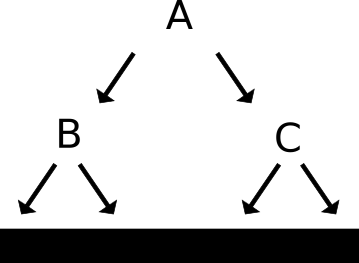
\includegraphics[scale=0.2]{OBB_Tree.png} 
\end{center}
\hrule
\begin{center}
\includegraphics[scale=0.18]{OBB_A.png}
\includegraphics[scale=0.18]{OBB_BC.png}
\includegraphics[scale=0.18]{OBB_DEFG.png} \\
\end{center}

\end{frame}

%--- Frame 11 ----------------%
\begin{frame}
\frametitle{DAG-MCNP Workflow}
\begin{center}
\includegraphics[scale=0.23, trim = 40 200 0 0]{DAGMC_Wrkflw5.png}
\end{center}
\end{frame}

%--- Frame 12 ----------------%
\begin{frame}
\frametitle{DAG-MCNP Workflow}
\begin{center}
\includegraphics[scale=0.23, trim = 40 200 0 0]{DAGMC_Wrkflw6.png}
\end{center}
\end{frame}


%--- Frame 13 ----------------%
\begin{frame}
\frametitle{DAG-MCNP Challenges}
\begin{itemize}
\vfill
\item Quality of CAD geometry
	\begin{itemize}
	\item small gaps \& overlaps
	\item lost particles
	\end{itemize}
\vfill
\item Human efficiency gains limited
	\begin{itemize}
	\item unique DAG-MCNP skill set required
	\end{itemize}
\vfill
\item DAG-MCNP-specific challenges
	\begin{itemize}
	\item Inconsistent faceting
	\item Robustness of tracking algorithm relies heavily on CAD
	\end{itemize}
\end{itemize}
\end{frame}

%--- Frame 14 ----------------%
\begin{frame}
\frametitle{DAG-MCNP Challenges}
\begin{itemize}
\vfill

\item Quality of CAD geometry
	\begin{itemize}
	\color{red}
	\item small gaps \& overlaps
	\item lost particles
	\end{itemize}
\vfill
\item Human efficiency gains limited
	\begin{itemize}
	\item unique DAG-MCNP skill set required	
	\end{itemize}
\vfill
\item DAG-MCNP-specific challenges
	\begin{itemize}
	\item Inconsistent faceting
	\item Robustness of tracking algorithm relies heavily on CAD
	\end{itemize}
\end{itemize}
\end{frame}



%--- Frame 15 ---------------%
\begin{frame}
\frametitle{make\_watertight}
\begin{itemize}
\item Developed by Brandon Smith (2011)
\item purpose is to seal faceted CAD models using geometric information provided by CGM
\item Algorithm became incompatible with external software infratstructure and has recently been refactored
\item Improves the topological soundness and accuracy of geometric models
\item Recent success in applying make\_watertight to complex geometries
\end{itemize}
\end{frame}

%--- Frame 16 ---------------%
\begin{frame}
\frametitle{make\_watertight}
\begin{itemize}
\item Seals small gaps in volumes using faceted geometry curves
\end{itemize}
\begin{center}
\includegraphics[scale=0.25, trim = 0 200 0 0 ]{cyl_loop_close.png}

\end{center}

\end{frame}


%--- Frame 17 ---------------%
\begin{frame}
\frametitle{make\_watertight}

\begin{center}


\includegraphics[scale=0.25, trim = 0 0 0 0 ]{cyl_loop_close.png}
\vfill 
before: 332 verticess \\ after: 190 vertices
\end{center}
\end{frame}


%--- Frame 18 ---------------%
\begin{frame}
\frametitle{make\_watertight}

\begin{itemize}
\vfill
\item By definition faceted models are not watertight
	\begin{itemize}
	\item CGM faceting engine in dagmc\_preproc (same as Cubit's)
	\item Surfaces do not share skin vertices
	\item Doesn't mean the model won't work
	\item Inherently has topological ambiguities
	\end{itemize}
\vfill
\item Algorithm makes topological changes to the model for watertightness

\end{itemize}
\includegraphics[scale=0.45, trim = -100 0 0 300 ]{stitch00.png}

\end{frame}

%--- Frame 19 ---------------%
\begin{frame}
\frametitle{make\_watertight}
\begin{itemize}
\item applies faceted geometric information from CGM to remove topological ambiguity from the model
\end{itemize}
\includegraphics[scale=0.4, trim = 20 50 0 0]{sealing_ex.png}
\end{frame}




%--- Frame 20 ---------------%
\begin{frame}
\frametitle{Recent Success}

ARIES Model
\begin{center}
\includegraphics[scale=0.3]{sic.png}
\end{center}
was losing 1 in 10k particles before sealing
\end{frame}


%--- Frame 21 ---------------%
\begin{frame}
\frametitle{Recent Success}

ARIES Model - zero lost particles in 10\textsuperscript{9}
\begin{center}
\scalebox{-1}[1]{\includegraphics[scale=0.3]{sic-bottom.png}}
\end{center}

\end{frame}

%--- Frame 22 ---------------%
\begin{frame}
\frametitle{Recent Success}
ARIES Model
\begin{center}
\includegraphics[scale=0.25]{Coolant_Channels.png}
\end{center}
\end{frame}


%--- Frame 22 ---------------%
\begin{frame}
\frametitle{Recent Success}
ARIES Model
\begin{center}
\includegraphics[scale=0.25]{Channel_Corner_Zoomed.png}
\end{center}
\end{frame}

%--- Frame 22 ---------------%
\begin{frame}
\frametitle{Recent Success}
ARIES Model
\begin{center}
\includegraphics[scale=0.25]{Channel_corner_broken_2.png}
\end{center}
\end{frame}

%--- Frame 22 ---------------%
\begin{frame}
\frametitle{Recent Success}
ARIES Model
\begin{center}
\includegraphics[scale=0.25]{Channel_corner_broken_3.png}
\end{center}
\end{frame}


%--- Frame 22 ---------------%
\begin{frame}
\frametitle{Recent Success}

ITER Blanket Lite
 - zero lost particles in 10\textsuperscript{8}
\begin{center}
\scalebox{-1}[1]{\includegraphics[scale=0.3]{blanketlitemodel.png}}
\end{center}

\end{frame}

%--- Frame 23 ---------------%
\begin{frame}
\frametitle{Recent Success}

ITER Blanket Lite
\begin{center}
\scalebox{-1}[1]{\includegraphics[scale=0.3]{blanketlitemodel_detail.png}}
\end{center}

\end{frame}

%--- Frame 24 ---------------%
\begin{frame}
\frametitle{Recent Success}

NASA Module
\begin{center}
\includegraphics[scale=0.3]{nasa_module.png}
\end{center}
5 surfaces unsealed
\end{frame}

%--- Frame 25 ---------------%
\begin{frame}
\frametitle{Recent Success}

NASA Module
\begin{center}
\includegraphics[scale=0.35]{bad_faceting.png}
\end{center}
\end{frame}

%--- Frame 26 ---------------%
\begin{frame}
\frametitle{Recent Success}

NASA Module
\begin{center}
\includegraphics[scale=0.35]{bad_facets.png}
\end{center}
\end{frame}

%--- Frame 27 ---------------%
\begin{frame}
\frametitle{Limitations of make\_watertight}
\begin{itemize}
\item Won't fix large-scale faceting issues
\item Can't fix bad geometry
\end{itemize}
\begin{center}
\textbf{tolerant tracking}
\vfill
\includegraphics[scale=0.2, trim = 0 0 100 100]{VolOverlap.png}
max tolerance: 10\textsuperscript{-3} cm
\end{center}

\end{frame}

%--- Frame 28 ---------------%
\begin{frame}
\frametitle{Future work}
\begin{itemize}
\item Integrate make\_watertight into the DAG-MCNP workflow
\item Separate faceting from CGM
	\begin{itemize}
	\item creates freedom to facet geometry features case by case
	\end{itemize}
\item Improve DAG-MCNP faceting performance
	\begin{itemize}
	\item high valence vertices
	\end{itemize}
\end{itemize}
\includegraphics[scale=0.25, trim = 0 200 0 0 ]{DAGMC_Wrkflw7.png}
\end{frame}



%--- Frame 29 ---------------%
\begin{frame}
\frametitle{High valence vertices}
\begin{itemize}
\item Defeats the nature of the OBB tree
\item Typically stems from some kind of geometry flaw
\end{itemize}
\begin{center}
\includegraphics[scale=0.26]{high_valence_vert.png}
\end{center}
\begin{itemize}
\item how to avoid these?
\end{itemize}
\end{frame}


%--- Frame 30 ---------------%
\begin{frame}
\frametitle{High valence vertices}
\begin{center}
\includegraphics[scale=0.6, trim = 0 0 0 300]{HV_1.png}
\end{center}
\end{frame}


%--- Frame 31 ---------------%
\begin{frame}
\frametitle{High valence vertices}
\begin{center}
\includegraphics[scale=0.6, trim = 0 0 0 300]{HV_2.png}
\end{center}
\end{frame}

%--- Frame 32 ---------------%
\begin{frame}
\frametitle{High valence vertices}
\begin{center}
\includegraphics[scale=0.6, trim = 0 0 0 300]{HV_4.png}
\end{center}
\end{frame}

%--- Frame 33 ---------------%
\begin{frame}
\frametitle{High valence vertices}
\begin{center}
\includegraphics[scale=0.6, trim = 0 0 0 300]{HV_4_boxes2.png}
\end{center}
\end{frame}

%--- Frame 34 ---------------%
\begin{frame}
\frametitle{Summary}
\begin{itemize}
\item DAG-MCNP has become more robust with the revival of make\_watertight

\item There has been success in sealing complex models for analysis

\item Further robustness in DAG-MCNP faceting is desired
\end{itemize}
\begin{center}
\includegraphics[scale=0.2]{InitialGraphImpact_postmw.png}
\end{center}

\end{frame}


%--- Frame 35 ---------------%
\begin{frame}
\frametitle{Thank you!}

\begin{center}
Questions?
\end{center}
Special thank you to:\\
Paul Wilson \\
Andrew Davis
\end{frame}


\end{document}


